\chapter{\label{ch:dev}Development practices}

As this is a new software project, we invested significant effort in setting
up a development infrastructure to ensure our work is tracked,
thoroughly and continually tested, and incrementally improved and documented.
To this end, we have adopted best practices for software development used by
many successful open source projects \cite{millman2014}.

\section{\label{sec:vc}Version control and code review}

We use Git\footnote{\url{http://git-scm.com}} as our version control system
(VCS) and GitHub\footnote{\url{https://github.com}} as the public hosting
service for our official \texttt{upstream} repository
(\url{https://github.com/statlab/permute}).  Each developer has their own copy,
or fork, of the \texttt{upstream} repository.  We each work on our own
repositories and use the \texttt{upstream} repository as our coordination or
integration repository.

Git allows us to track and manage how our code changes over time as well as
review all new functionality before merging it into the \texttt{upstream}
repository.  To get new code integrated in the \texttt{upstream} repository, we
use GitHub's \emph{pull request} mechanism.  This enables us to review code
before integrating it.  In the following section, I describe how we automate
our testing to generate reports for all pull requests.  This way we can reduce
the risk that changes to our code break existing functionality.  Once a pull
request is reviewed and accepted, it is merged into the \texttt{upstream}
repository.

Requiring all new code to undergo review provides several benefits.  Code
review increases the quality and consistency of our codebase.  It helps
maintain a high level of test coverage (see below).  Moreover, it also
helps keep the development team aware of the work other team members are
doing.  While we are currently a small team and we meet regularly, having
the code review system in place will make it easier for new people to
contribute as well as capturing our design discussions and decisions for
future reference.

\section{\label{sec:test}Testing and continuous integration}

We use the \texttt{nose} testing framework for automating our testing
procedures.\footnote{\url{https://nose.readthedocs.org}}  This is the standard
testing framework used by the core packages in the scientific Python ecosystem.
Automating the tests allows us to monitor a proxy for code correctness when
making changes as well as simplifying the code review process for new code.
Without automated testing, we would have to manually test all the code every
time a change is proposed.  The \texttt{nose} testing framework simplifies test
creation, discovery, and running. It has an extensive set of plugins to add
functionality for coverage reporting, test annotation, profiling, as well as
inspecting and testing documentation.

\begin{figure}
  \begin{centering}
    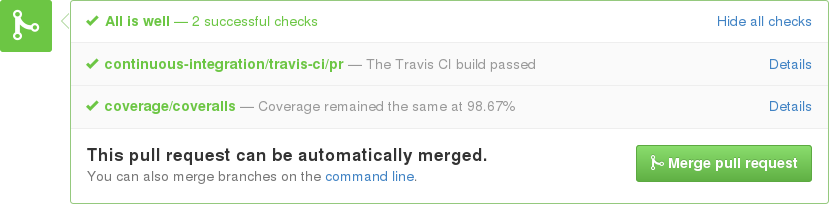
\includegraphics[width=\textwidth]{fig/pull-request-ci.png}\par
  \end{centering}

  \caption{\label{fig:pull-request}Pull request and continuous integration.}
\setlength{\leftskip}{1cm}
\setlength{\rightskip}{1cm}
\small
Each pull request triggers an automated system to run the  full test suite on
the updated codebase.
This means that when you go to review a pull request you can immediately see
whether the change breaks any of the tests as well as whether the new
code decreases the overall test coverage.
For example, the above report indicates that the associated pull request does not
break existing code and does not change our test coverage.
\end{figure}

Our goal is to test every line of code.  For example, not only do we want to
test every function in our package, but if a specific function has internal
logic we want to test each possible execution path through the function.
Having tested each line of code increases our confidence in our codebase, but
more importantly provides us some measure of assurance that changes we make do
not break existing code.  It also increases our confidence that new code works,
which reduces the friction of accepting contributions.  Currently over 98\% of
\texttt{permute}'s lines of code get executed at least once by our test system.

We have configured Travis CI\footnote{\url{https://travis-ci.org}} and
\texttt{coveralls}\footnote{\url{https://coveralls.io}} to be automatically
triggered whenever a commit is made to a pull request or the upstream master
(see Figure~\ref{fig:pull-request}).  These systems then run the full
test suite  using different versions of our dependencies (e.g., Python 2.7 and
3.4) every time a new commit is made to a repository or pull request.
%This
%means that when you go to review a pull request you can immediately see a full
%report of whether the change breaks any of the tests as well as whether the new
%code decreases the overall test coverage.

\section{\label{sec:doc}Documentation}

We use Sphinx\footnote{\url{http://sphinx-doc.org}} as our documentation system
and already have good developer documentation and the foundation for
high-quality user documentation. Sphinx is the standard documentation system
for Python projects and is used by all the core scientific Python packages.
We use Python docstrings and follow the NumPy docstring
standard\footnote{\url{https://github.com/numpy/numpy/blob/master/doc/HOWTO\_DOCUMENT.rst.txt}}
to document all the modules and functions in \texttt{permute}.  Using Sphinx
and some NumPy extensions, we have a system for autogenerating the project
documentation (as HTML or PDF) using the docstrings as well as stand-alone text
written in a light-weight markdown-like language, called
reStructuredText\footnote{\url{http://docutils.sourceforge.net/rst.html}}.
This system enables us to easily embed references, figures, code that is
auto-run during documentation generation, as well as mathematics using \LaTeX.

\section{\label{sec:release}Release management}

Our development workflow ensures that the official \texttt{upstream} repository
is always stable and ready for use.  This means anyone can get our official
upstream master at any point, install it and start using it.  We also make
official releases available as source tarballs as well as Python
built-packages\footnote{Presently our code is pure Python, but we release
Python wheels.  Wheels are the new standard built-package format for Python.}
uploaded to the Python Package Index, or PyPI,\footnote{PyPI is the Python
equivalent of The Comprehensive R Archive Network (CRAN).} with release
announcements posted to our mailing list.  To install the latest release of
\texttt{permute} and its dependencies, type the following command from a shell
prompt (assuming you have Python and a recent version of pip): 

\texttt{\$ pip install permute}
